\documentclass{article}

\usepackage{fancyhdr}
\usepackage{extramarks}
\usepackage{amsmath}
\usepackage{amsthm}
\usepackage{amsfonts}
\usepackage{amssymb}
\usepackage{xparse}
\usepackage{tikz}
\usepackage{graphicx}
\usepackage[plain]{algorithm}
\usepackage{algpseudocode}
\usepackage{listings}
\usepackage{hyperref}
\usepackage[per-mode = fraction]{siunitx}
\usepackage{calc}

\usetikzlibrary{automata,positioning}

\hypersetup{
    colorlinks=true,
    linkcolor=blue,
    filecolor=magenta,
    urlcolor=blue,
    }

\urlstyle{same}

%
% Basic Document Settings
%

\topmargin=-0.45in
\evensidemargin=0in
\oddsidemargin=0in
\textwidth=6.5in
\textheight=9.0in
\headsep=0.25in

\linespread{1.1}

\pagestyle{fancy}
\lhead{\hmwkAuthorName}
\chead{\hmwkClass\ (\hmwkClassInstructor,\ \hmwkClassTime): \hmwkTitle}
\rhead{\firstxmark}
\lfoot{\lastxmark}
\cfoot{\thepage}

\renewcommand\headrulewidth{0.4pt}
\renewcommand\footrulewidth{0.4pt}

\setlength\parindent{0pt}
\allowdisplaybreaks
%
% Title Page
%

\title{
	\vspace{2in}
	\textmd{\textbf{\hmwkClass:\ \hmwkTitle}}\\
	\normalsize\vspace{0.1in}\small{Due\ on\ \hmwkDueDate\ at \hmwkDueTime}\\
	\vspace{0.1in}\large{\textit{\hmwkClassInstructor,\ \hmwkClassTime}}
	\vspace{3in}
}
\author{\textbf{\hmwkAuthorName}}
\date{\hmwkCompletionDate}

%
% Create Problem Sections
%

\newcommand{\enterProblemHeader}[1]{
	\nobreak\extramarks{}{Problem #1 continued on next page\ldots}\nobreak{}
	\nobreak\extramarks{Problem #1 (continued)}{Problem #1 continued on next page\ldots}\nobreak{}
}

\newcommand{\exitProblemHeader}[1]{
	\nobreak\extramarks{Problem #1 (continued)}{Problem #1 continued on next page\ldots}\nobreak{}
	\nobreak\extramarks{Problem #1}{}\nobreak{}
}

%
% Homework Problem Environment
%
\NewDocumentEnvironment{hwkProblem}{m m s}{
	\section*{Problem #1: #2}
	\enterProblemHeader{#1}
	\setcounter{partCounter}{1}
}{
	\exitProblemHeader{#1}
	\IfBooleanF{#3} % if star, no new page
		{\newpage}
}

% Alias for the Solution section header
\newcommand{\hwkSol}{\vspace{\baselineskip / 2}\textbf{\Large Solution}\vspace{\baselineskip / 2}}

% Alias for the Solution Part subsection header
\newcounter{partCounter}
\newcommand{\hwkPart}{
	\vspace{\baselineskip / 2}
	\textbf{\large Part \Alph{partCounter}}
	\vspace{\baselineskip / 2}
	\stepcounter{partCounter}
}

%
% Various Helper Commands
%

% Such That
\newcommand{\st}{\text{s.t.}}

% Useful for algorithms
\newcommand{\alg}[1]{\textsc{\bfseries \footnotesize #1}}

% For derivatives
\newcommand{\deriv}[1]{\frac{\mathrm{d}}{\mathrm{d}x} (#1)}

% For partial derivatives
\newcommand{\pderiv}[2]{\frac{\partial}{\partial #1} (#2)}

% Integral dx
\newcommand{\dx}{\mathrm{d}x}
\newcommand{\dy}{\mathrm{d}y}

% Probability commands: Expectation, Variance, Covariance, Bias
\newcommand{\e}[1]{\mathrm{e}#1}
\newcommand{\E}{\mathrm{E}}
\newcommand{\Var}{\mathrm{Var}}
\newcommand{\Cov}{\mathrm{Cov}}
\newcommand{\Bias}{\mathrm{Bias}}

% Defining Units that are not in the SI base
\DeclareSIUnit\bar{bar}
\DeclareSIUnit\ft{ft}
\DeclareSIUnit\dollar{\$}
\DeclareSIUnit\cent{\text{\textcent}}
\DeclareSIUnit\c{\degreeCelsius}

% Code Listing config
\usepackage{xcolor}
\definecolor{codegreen}{rgb}{0,0.6,0}
\definecolor{codegray}{rgb}{0.5,0.5,0.5}
\definecolor{codepurple}{rgb}{0.58,0,0.82}
\definecolor{backcolour}{rgb}{0.95,0.95,0.92}
\lstdefinestyle{overleaf}{
	% backgroundcolor=\color{backcolour},
	commentstyle=\color{codegreen},
	keywordstyle=\color{magenta},
	numberstyle=\tiny\color{codegray},
	stringstyle=\color{codepurple},
	basicstyle=\ttfamily\footnotesize,
	breakatwhitespace=false,
	breaklines=true,
	captionpos=b,
	keepspaces=true,
	numbers=left,
	numbersep=5pt,
	showspaces=false,
	showstringspaces=false,
	showtabs=false,
	tabsize=4
}

\usepackage[latte]{catppuccinpalette}
\lstdefinestyle{catppuccin}{
	breaklines=true,
	keepspaces=true,
	numbers=left,
	numbersep=5pt,
	showspaces=false,
	showstringspaces=false,
	breakatwhitespace=true,
	tabsize=4,
	stringstyle = {\color{CtpGreen}},
	commentstyle={\color{CtpOverlay1}},
	basicstyle = {\small\color{CtpText}\ttfamily},
	keywordstyle = {\color{CtpMauve}},
	keywordstyle = [2]{\color{CtpBlue}},
	keywordstyle = [3]{\color{CtpYellow}},
	keywordstyle = [4]{\color{CtpLavender}},
	keywordstyle = [5]{\color{CtpPeach}},
	keywordstyle = [6]{\color{CtpTeal}}
}

\lstset{style=catppuccin}


%
% Homework Details
%   - Title
%   - Due date
%   - Due time
%   - Course
%   - Section/Time
%   - Instructor
%   - Author
%

\newcommand{\hmwkTitle}{Homework 03}
\newcommand{\hmwkSubTitle}{}
\newcommand{\hmwkDueDate}{March 03th, 2025}
\newcommand{\hmwkDueTime}{03:30 PM}
\newcommand{\hmwkClass}{ENRE 447 - 0101}
\newcommand{\hmwkClassTime}{03:30 PM}
\newcommand{\hmwkClassInstructor}{Dr. Groth}
\newcommand{\hmwkAuthorName}{\textbf{Vai Srivastava}}
\newcommand{\hmwkCompletionDate}{\today}

\begin{document}

\maketitle

\pagebreak

\begin{hwkProblem}{1}{}

	The following data represent times to failure (in hours) for 20 mechanical devices.
	\begin{center}
		\begin{tabular}{llllllllll}
			4 & 7 & 8 & 12 & 19 & 27 & 50 & 65 & 66 & 69 \\
			71 & 73 & 75 & 91 & 107 & 115 & 142 & 166 & 184 & 192 \\
		\end{tabular}
	\end{center}
	\begin{enumerate}
		\item Find the MTTF and Variance of the failure times.
		\item Develop an empirical probability distribution and histogram for the data.
	\end{enumerate}

	\hwkSol

	\hwkPart
	\begin{align*}
		\sum_{i=1}^{20} t_i &= 4+7+\cdots+184+192 = 1543 \\
		\bar{t} &= \frac{1543}{20} \approx 77.15 \\
		\text{MTTF} = 77.15 \text{ hours}. \quad \qed \\
		\sigma^2 &= \frac{1}{20}\sum_{i=1}^{20} t_i^2 - \bar{t}^2 \\
		\frac{1}{20}\sum_{i=1}^{20} t_i^2 &\approx 9229.75,\quad \bar{t}^2\approx 5952.12 \\
		\sigma^2 \approx 9229.75 - 5952.12 = 3277.63 \text{ (hours)}^2. \quad \qed
	\end{align*}

	\hwkPart

	\begin{figure}[H]
		\centering
		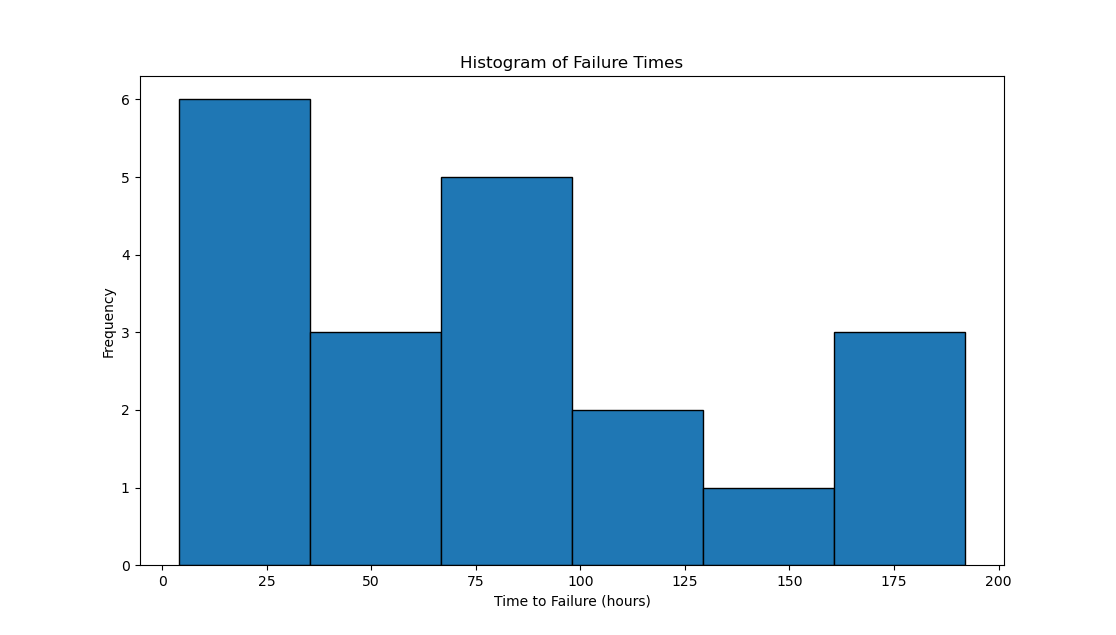
\includegraphics[width=0.8\textwidth]{./images/s01b1.png}
	\end{figure}

	\begin{figure}[H]
		\centering
		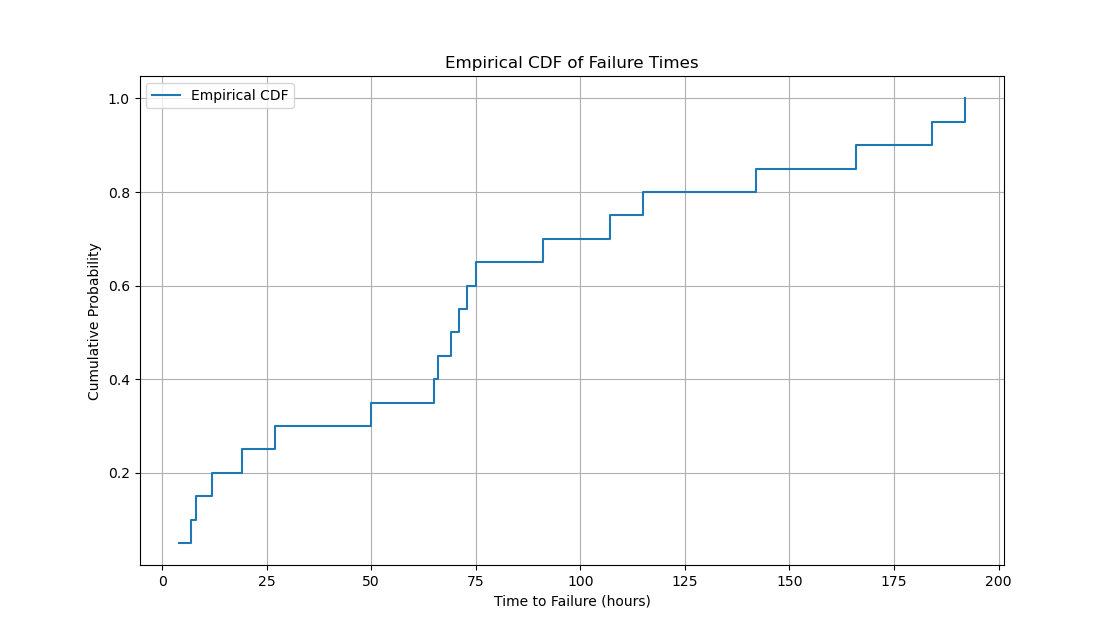
\includegraphics[width=\textwidth]{./images/s01b2.png}
	\end{figure}

	\lstinputlisting[language=python, caption={Python code for HW03 P01B}, label={lst:s01b}]{./code/s01b.py}

\end{hwkProblem}

\begin{hwkProblem}{2}{}

	The histogram below shows the distribution of the diameters of the heads of rivets manufactured by a company. Compute the mean and variance of the diameter.
	\begin{figure}[H]
	  \centering
	  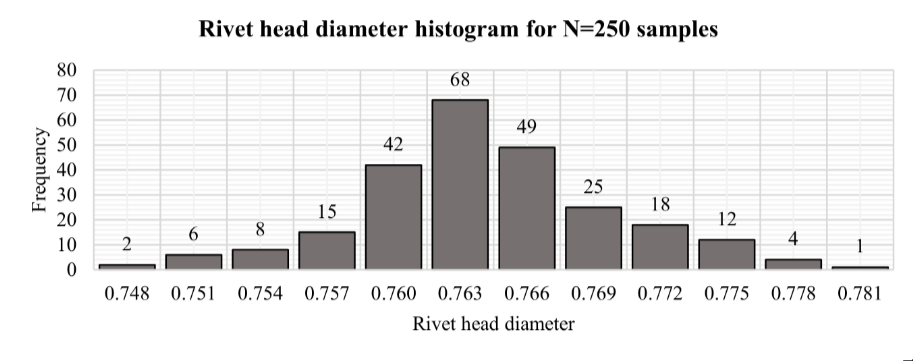
\includegraphics[width=0.8\textwidth]{./images/p02.png}
	\end{figure}
	\begin{center}
		\begin{tabular}{lcccccccccccc}
			Diameter: & 0.748 & 0.751 & 0.754 & 0.757 & 0.760 & 0.763 & 0.766 & 0.769 & 0.772 & 0.775 & 0.778 & 0.781 \\
			Frequency: & 2 & 6 & 8 & 15 & 42 & 68 & 49 & 25 & 18 & 12 & 4 & 1
		\end{tabular}
	\end{center}

	\hwkSol

	\begin{align*}
		\bar{x} &= \frac{1}{N}\sum_{i=1}^{12} t_{i}\Prob[t_{i}] = \frac{2(0.748)+6(0.751)+\cdots+4(0.778)+1(0.781)}{250} \approx 0.7642. \quad \qed \\
		\overline{x^2} &= \frac{1}{N}\sum_{i=1}^{12} t_{i}\Prob[t_{i}]^{2} = \frac{2(0.748^2)+6(0.751^2)+\cdots+1(0.781^2)}{250} \approx 0.58404 \\
		\sigma^2 &= \overline{x^2} - \bar{x}^2 \approx 0.58404 - (0.7642)^2 \approx 0.58404 - 0.58395 \approx 0.00009 \text{ (units)}^{2}. \quad \qed
	\end{align*}

\end{hwkProblem}

\begin{hwkProblem}{3}{}

	The sample mean life of ten car batteries is 102.5 months, with a standard deviation of 9.45 months. What are the 80\% confidence limits for the mean and standard deviation of a pdf that represents these batteries?

	\hwkSol

	\begin{align*}
		t_{0.10,9} &\approx 1.383 \\
		\text{Margin of Error} &= 1.383 \cdot \frac{9.45}{\sqrt{10}} \approx 1.383 \cdot 2.988 \approx 4.14 \\
		\text{CI for } \mu &: \quad 102.5 \pm 4.14,\quad (102.5-4.14,\;102.5+4.14) \approx (98.36,\;106.64). \quad \qed \\
		s^2 &= (9.45)^2 \approx 89.3025 \\
		\chi^2_{0.90,9} &\approx 14.684,\quad \chi^2_{0.10,9} \approx 5.226 \\
		\text{Lower variance limit} &= \frac{9 \cdot 89.3025}{14.684} \approx 54.73 \\
		\text{Upper variance limit} &= \frac{9 \cdot 89.3025}{5.226} \approx 153.80 \\
		\text{CI for } \sigma &: \quad \left(\sqrt{54.73},\sqrt{153.80}\right) \approx (7.40,\;12.40). \quad \qed
	\end{align*}

\end{hwkProblem}

\begin{hwkProblem}{4}{}

	The frequency distribution of time to establish the root causes of a failure by a group of experts is observed and given below. Test whether a normal distribution with known \( \sigma = 10 \) is an appropriate model for these data.
	\begin{center}
		\begin{tabular}{ll}
			\hline
			Time Interval (hour) & Obs. Freq. \\
			\hline
			\(45-55\) & 7 \\
			\(55-65\) & 18 \\
			\(65-75\) & 35 \\
			\(75-85\) & 28 \\
			\(85-95\) & 12 \\
			\hline
		\end{tabular}
	\end{center}

	\hwkSol

	\begin{align*}
		\bar{x} &= \frac{7\left(\frac{45+55}{2}\right)+\cdots+12\left(\frac{85+95}{2}\right)}{7+\cdots+12} = \frac{350+1080+2450+2240+1080}{100} = \frac{7200}{100} = 72 \\
		P(45 \le X \le 55) &= \Phi\Bigl(\frac{55-72}{10}\Bigr)-\Phi\Bigl(\frac{45-72}{10}\Bigr) \\
				   &\approx \Phi(-1.7)-\Phi(-2.7) \approx 0.0446-0.0035 = 0.0411 \\
		E_1 &= 100 \cdot 0.0411 \approx 4.11 \\
		P(55 \le X \le 65) &\approx 0.1974,\quad E_2 \approx 19.74 \\
		P(65 \le X \le 75) &\approx 0.3759,\quad E_3 \approx 37.59 \\
		P(75 \le X \le 85) &\approx 0.2853,\quad E_4 \approx 28.53 \\
		P(85 \le X \le 95) &\approx 0.0861,\quad E_5 \approx 8.61 \\
		\chi^2 &= \frac{(7-4.11)^2}{4.11}+\frac{(18-19.74)^2}{19.74}+\frac{(35-37.59)^2}{37.59}+\frac{(28-28.53)^2}{28.53}+\frac{(12-8.61)^2}{8.61} \\
		       &\approx \frac{(2.89)^2}{4.11}+\frac{(-1.74)^2}{19.74}+\frac{(-2.59)^2}{37.59}+\frac{(-0.53)^2}{28.53}+\frac{(3.39)^2}{8.61} \\
		       &\approx 2.03+0.15+0.18+0.01+1.34 \approx 3.71 \\
		\text{df} &= 5 - 1 - 1 = 3 \\
		\chi^2_{0.05,3} &\approx 7.815,\quad 3.71 < 7.815. \quad \qed
	\end{align*}

\end{hwkProblem}

\begin{hwkProblem}{5}{}

	A sample of 50 digits using a random number generator yielded the following data. Is there any reason to doubt the digits are uniformly distributed? Use a Chi-Square test and significance level of 0.05 to test.
	\begin{center}
		\begin{tabular}{lllllclllll}
			Digit: & 0 & 1 & 2 & 3 & 4 & 5 & 6 & 7 & 8 & 9 \\
			Frequency: & 4 & 8 & 8 & 4 & 10 & 3 & 2 & 2 & 4 & 5 \\
		\end{tabular}
	\end{center}

	\hwkSol

	\begin{align*}
		E &= \frac{50}{10} = 5 \\
		\chi^2 &= \sum_{i=0}^{9} \frac{(O_i-5)^2}{5} \\
		       &= \frac{(4-5)^2+(8-5)^2+\cdots+(4-5)^2+(5-5)^2}{5} \\
		       &= \frac{1+9+\cdots+1+0}{5} = \frac{69}{5} \approx 13.8 \\
		\text{df} &= 10 - 1 = 9 \\
		\chi^2_{0.05,9} &\approx 16.92,\quad 13.8 < 16.92. \quad \qed
	\end{align*}

\end{hwkProblem}

\begin{hwkProblem}{6}{}

	Consider the following time to failure data with the ranked value of \( t_{i} \). Use the K-S test to test the hypothesis that the data fit a normal distribution.
	\begin{center}
		\begin{tabular}{l|llllllllll}
			\hline
			Event & 1 & 2 & 3 & 4 & 5 & 6 & 7 & 8 & 9 & 10 \\
			\hline
			Time to Failure (hour) & 10.3 & 12.4 & 13.7 & 13.9 & 14.1 & 14.2 & 14.4 & 15.0 & 15.9 & 16.1 \\
			\hline
		\end{tabular}
	\end{center}

	\hwkSol

	\begin{align*}
		\bar{t} &= \frac{10.3+12.4+\cdots+15.9+16.1}{10} = \frac{140.0}{10} = 14.0 \\
		s &\approx 1.686 \\
		\text{For each } t_i,\quad F(t_i) &= \Phi\left(\frac{t_i-14.0}{1.686}\right) \\
		\text{Empirical CDF at } t_i &= \frac{i}{10} \\
		D &= \max_{1\le i\le 10} \left|F(t_i)-\frac{i}{10}\right| \approx 0.129 \\
		D_{0.05} &\approx \frac{1.36}{\sqrt{10}} \approx 0.430 \\
		0.129 &< 0.430. \quad \qed
	\end{align*}

\end{hwkProblem}

\end{document}
